\documentclass[twoside,letterpaper,12pt]{report}
\usepackage[spanish,backgroundcolor=green,textsize=small]{todonotes}
\usepackage[margin=2cm]{geometry}
\usepackage[utf8x]{inputenc}
\usepackage[spanish]{babel}
\usepackage{plain}
\usepackage{amsmath}
\usepackage{graphicx}
\usepackage{wrapfig}
\usepackage{parskip}
\usepackage{nomencl}
\setlength{\parindent}{15pt}
\usepackage{hyperref}
\hypersetup{
  colorlinks=true,
  linkcolor=black,          % color of internal links (change box color with linkbordercolor)
  citecolor=black,        % color of links to bibliography
  filecolor=black,      % color of file links
  urlcolor=black           % color of external links }
}

\title{
	Proyecto de Grado\\[0.5cm]
	Instalación, Implementación y Uso de las librerías Boost y su aplicación en recorrido de grafos para la supercomputadora Apolo
}

\vspace{1cm}

\author{
	Autor:\\[0.3cm]
	Sergio Andrés Monsalve Castañeda\\
	Código: 200410061010\\
	smonsal3@eafit.edu.co\\[0.7cm]
	Asesor: \\[0.3cm]
	Juan Guillermo Lalinde Pulido\\
	jlalinde@eafit.edu.co\\
	2619500 ext 9588%\\[1cm]
}

\date{
	\today \\[0.5cm]
	
\includegraphics[width=0.25\textwidth]{aux/logo_eafit} 
}

\begin{document}

% Primera Portada _____________________________________________________________________

\maketitle

% Segunda Portada _____________________________________________________________________

\thispagestyle{empty} % Esta pagina no se numera
\begin{center}
\textbf{{\Large Instalación, Implementación y Uso de las librerías Boost y su aplicación en recorrido de grafos para la supercomputadora Apolo}}\\[3cm]
{\Large Sergio Andrés Monsalve Castañeda} \\ {\large \textit{smonsal3@eafit.edu.co}}\\[2.5cm]
%{\large\emph{\textbf{Trabajo de grado presentado como requisito }}}\\
%\emph{\textbf{parcial  para optar al t\'itulo de Ingeniero Físico}}}\\[3cm]

{\large \textbf{Asesor:} \\ Doctor Juan Guillermo Lalinde Pulido}\\[3cm]

Ingeniería de Sistemas \\ Departamento de Informática y Sistemas  \\ Escuela de Ingeniería \\ Universidad EAFIT \\ Medellín, Colombia.\\
2013

\end{center}
\pagebreak

%------------------------- Aceptación --------------------------------%

\begin{flushright}
	Nota de aceptación\\
	\vspace{1cm}
	\rule{\textwidth}{1pt}\\
	\vspace{1cm}
	\rule{\textwidth}{1pt}\\
	\vspace{1cm}
	\rule{\textwidth}{1pt}\\
	\vspace{1.3cm}
	Presidente del jurado\\
	\vspace{1cm}
	\rule{\textwidth}{1pt}\\
	\vspace{1.3cm}
	Jurado\\
	\vspace{1cm}
	\rule{\textwidth}{1pt}\\
	\vspace{1.3cm}
	Jurado\\
	\vspace{1cm}
	\rule{\textwidth}{1pt}\\
	\vspace{2.5cm}
	\rule{\textwidth}{1pt}\\
	\vspace{.8cm}
	Ciudad y Fecha
\end{flushright}
\thispagestyle{empty}
\pagebreak


%---------------------- Tabla de contenido ---------------------------%

	\pdfbookmark[1]{\contentsname}{}
	\tableofcontents
	\cleardoublepage \phantomsection
	%\newpage
	\listoftables
	\addcontentsline{toc}{section}{\protect\numberline{}\listtablename}
	%\pdfbookmark[1]{Lista de tablas}{}
	\cleardoublepage \phantomsection
	%\newpage
	%\listfigurename
	\listoffigures
	\addcontentsline{toc}{section}{\protect\numberline{}\listfigurename}
	%\pdfbookmark[1]{Lista de figuras}{}
	\cleardoublepage \phantomsection
	%\newpage
	% \printnomenclature[2cm] %% Imprime la nomenclatura
	\addcontentsline{toc}{section}{\protect\numberline{}\nomname}
	%\pdfbookmark[1]{Lista de abreviaturas y símbolos}{}



\begin{abstract}

	Existe una gran cantidad de problemas que debido a su complejidad no es posible resolver, sea porque requieren mucho tiempo o la complejidad de estos esta tal que los hace inviables, adicionalmente cada vez surgen nuevos problemas, aun mas complejos. 

	Con el crecimiento de la capacidad computacional ya es posible abordar algunos de ellos que antes hubieran tomado mucho tiempo o simplemente no hubiese sido posible resolver. 

	Dentro de este amplia gama de problemas, existen un subcojunto particular que pueden ser modelados mediante la teoría de grafos, una gran herramienta que ofrece las ciencias de la computación.

	Aunque los algoritmos para grafos tienen una complejidad alta en general, existen algoritmos paralelos.

	En este proyecto se pretende instalar en Apolo, el supercomputador de EAFIT, la infraestructura básica para que un programador, utilizando las librerías BOOST para C++, pueda desarrollar rápidamente aplicaciones que aprovechen su capacidad computacional. 

	De esta manera se pretende beneficiar a la Comunidad Científica, Comunidad académica, Estudiantes de Ingeniería de Sistemas, Estudiantes de Ingenieria Matematica y en General a quien necesite realizar computo en un ambiente de computación de alto rendimiento, clusters computacionales, grafos en paralelo utilizando Boost, o requiera de una introducción a este tema.


\end{abstract}

\newpage

\renewcommand{\abstractname}{Agradecimientos}
\begin{abstract}

	En primer lugar quiero agradecer a Juan Guillermo Lalinde quien desde el inicio de mi carrera me inspiró y apoyó en grandes retos acádemicos. A Juan David Pineda por toda su paciencia para explicarme el funcionamiento de Apolo. Por ultimo agradezco a John Jairo Silva, Alejandro Gómez, Mateo Gómez, Jaime Pérez y John Mario Gutiérrez por sus multiples colaboraciones. 	

\end{abstract}

\newpage

\chapter{Introducción}
\section{Objetivos}

	\begin{itemize}
		\item Construir un manual para la instalación de las librerías de Boost.
		\item Generar Documentación sobre el manejo de las librerías de Boost.
		\item Correr códigos de ejemplo para la ejecución de las librerías de Boost.
	\end{itemize}

\section{Alcance y productos}
	\begin{itemize}
		\item Descripción de las librerías de Boost.
		\item Introducción a las librerías de utilización de grafos instaladas en Apolo.
		\item Introducción al manejo de Grafos con Boost (representación conceptual).
	\end{itemize}

\section{Productos}
	\begin{itemize}
		\item Manual de Instalacion de librerias Para Boost.
		\item Ejemplo en código documentado y manual de como hacer un programa utilizando Boost para grafos.	
		\item 
	\end{itemize}

\section{Usabilidad}

	Utilizar los GPS de los taxis para hacer análisis de la malla vial de la ciudad. 
	Movilización y Rutas óptimas para el recorrido de Bomberos, Ambulancias, Policía para la atención de emergencias y desastres

	Movilidad, Seguridad, Educación, Tecnología.



\chapter{Marco de Referencia}\label{ChapRef}

	\section{Computación Paralela}

	La computación paralela es el uso de múltiples recursos computacionales para resolver un problema o una necesidad de computo en particular. La computación paralela surge como respuesta ante la necesidad de incrementar los recursos, sea en procesador, memoria y así mejorar el tiempo de respuesta para problemas con alta complejidad computacional o alto volumen de análisis de datos. 

	El paradigma computacional tradicional ha sido de computación serial, donde una tarea es dividida en una serie finita de instrucciones que son ejecutada de forma secuencial, donde una sola instrucción es ejecutada en un momento dado. 

	La computación paralela rompe el paradigma anterior, buscando que en un momento dado se puedan ejecutar varias instrucciones, utilizando múltiples procesadores y una entidad que orqueste los mismos.  

	Para mayor información sobre Computación Paralela \cite{PCI}

	\cite{SC}

	\section{Apolo}

	\todo[inline,caption={TODO}]{Arquitectura de apolo. Redes.}

	\section{Grafos}

	Los grafos son abstracciones matemáticas que son útiles a la hora de resolver muchos tipos de problemas en las ciencias de la computación. 
	Un grafo es un conjunto ordenado 

	Nodos

	Vertices

	donde los vértices son relaciones 


	La aplicación de la teoría de grafos estudio de relaciones entre nodos. 



	\begin{figure}[H]
		\centering
		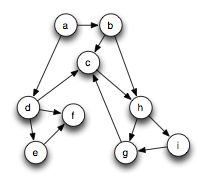
\includegraphics[width=0.5\textwidth]{aux/grafo}
		\caption[Estructura de un Grafo]{
		(tomada de \cite{BoostGrafos)}
		%\label{F-dimensions-emotion}
	\end{figure}


	\begin{figure}[H]
		\centering
		\includegraphics[width=0.5\textwidth]{aux/distributed_graph}
		\caption[Grafo Distribuido]{
		(tomada de \cite{BoostGrafos)}
		%\label{F-dimensions-emotion}
	\end{figure}
	
	

	\begin{figure}[H]
		\centering
		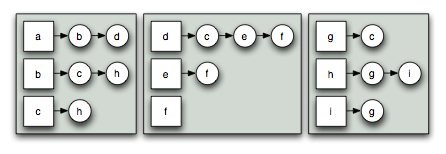
\includegraphics[width=0.5\textwidth]{aux/dist-adjlist}
		\caption[Grafo en lista de adyacencia]{
		(tomada de \cite{BoostGrafos)}
		%\label{F-dimensions-emotion}
	\end{figure}


	\begin{figure}[H]
		\centering
		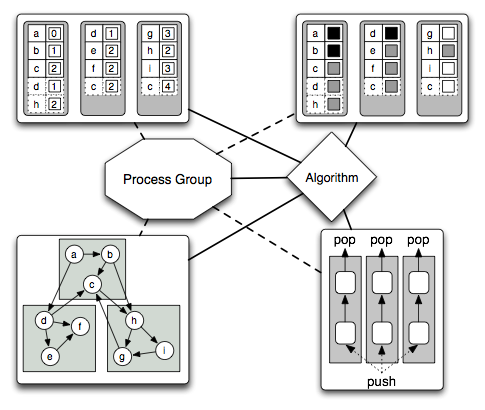
\includegraphics[width=0.5\textwidth]{aux/arquitectura_grafos}
		\caption[Aquitectura de Grafos]{
		(tomada de \cite{BoostGrafos)}
		%\label{F-dimensions-emotion}
	\end{figure}
	

	\section{C++}

	\section{MPI}

	\section{Boost}

	


	\section{Parallel Boost Graph Library}

	\begin{quotation}
		The Parallel Boost Graph Library is an extension to the Boost Graph Library (BGL) for parallel and distributed computing. It offers distributed graphs and graph algorithms to exploit coarse-grained parallelism along with parallel algorithms that exploit fine-grained parallelism, while retaining the same interfaces as the (sequential) BGL. Code written using the sequential BGL should be easy to parallelize with the parallel BGL. Visitors new to the Parallel BGL should read our architectural overview.\cite{wwwBoost} 
		\end{quotation} 

	\todo[inline,caption={TODO}]{Representacional}


\chapter{Virtualización}
\section{Virtualización de un cluster}

		\todo[inline,caption={TODO}]{Aca va la descripción de porque es importante virtualizar, para que se necesita y que es lo que se esta virtualizando.}


% http://galois.eafit.edu.co/vms/devenv/rocks-6.1/

La siguiente es la descripción de los pasos a seguir para la creación de un ambiente de pruebas paralelo virtualizado que simula el cluster de Apolo.\footnote{Estas instrucciones fueron probadas en un ambiente de Linux Fedora 18.}


\subsection{Configuración del Nodo Maestro}
\begin{enumerate}

\item Descargue e Instale VirtualBox Manager. \footnote{\url{https://www.virtualbox.org/wiki/Downloads}}

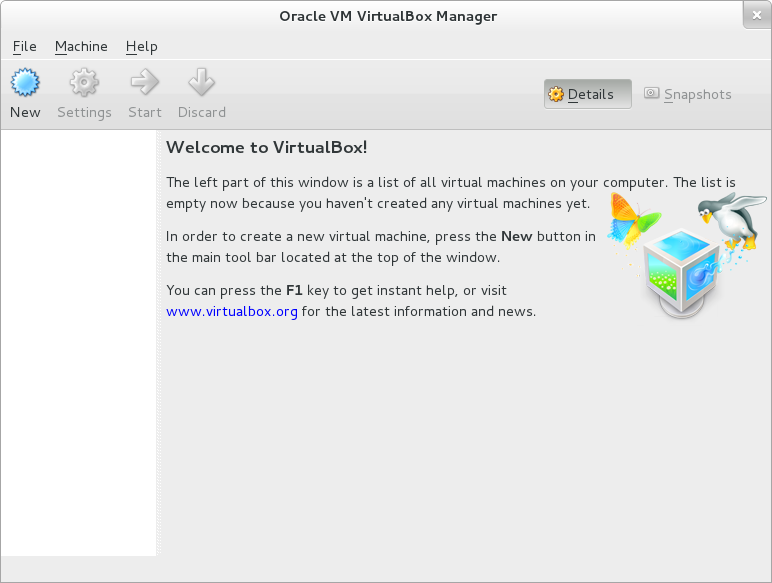
\includegraphics[width=0.5\textwidth]{aux/vb_instalado}

\item Descargar la imagen del Master.\footnote{\url{http://goo.gl/8eTJOr}}

\item Descargue el ``Extension Pack''. \footnote{\url{https://www.virtualbox.org/wiki/Downloads}}

\item Una vez instalado VirtualBox en su computador, proceda a instalar el Extensión Pack: 

	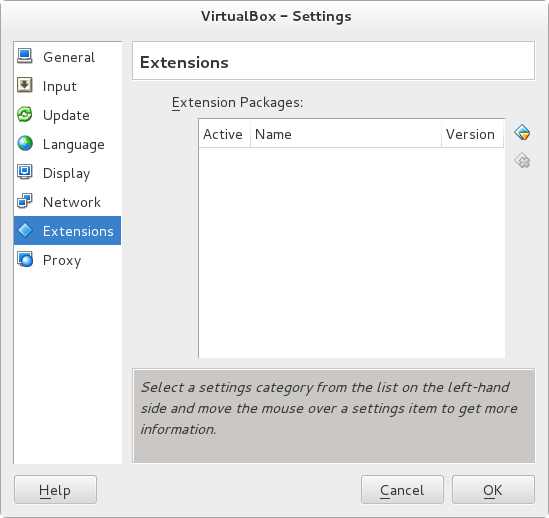
\includegraphics[width=0.5\textwidth]{aux/sinextensionpack}
	
\begin{itemize}


	\item En VirtualBox acceda al menú Archivo $\rightarrow$ Preferencias $\rightarrow$ Sección Extensiones $\rightarrow$ Proceda a instalar el ``Extension Pack''. 
	
	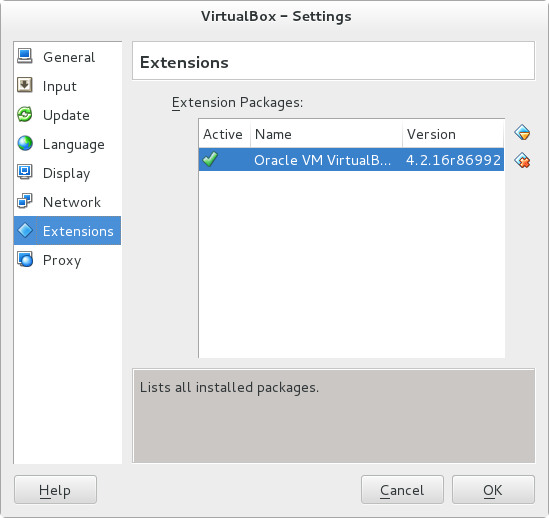
\includegraphics[width=0.5\textwidth]{aux/conextensionpack}

	\item Vaya a la sección Red $\rightarrow$ Adicione una red Sólo Anfitrión. Esta debe ser la primera interfaz de red de Sólo Anfitrión que se crea, si ya está creada por favor no cree otra adicional.


	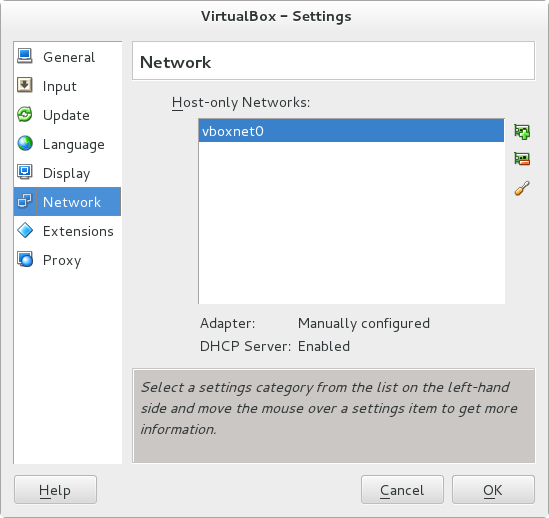
\includegraphics[width=0.5\textwidth]{aux/hostonly}
	

	\item Haga click en aceptar para finalizar la operación.

\end{itemize}

\item En VirtualBox, importe desde el Menú $\rightarrow$ Importar Appliance. Deje la configuración por defecto y \textbf{no} reinicialice la dirección MAC.


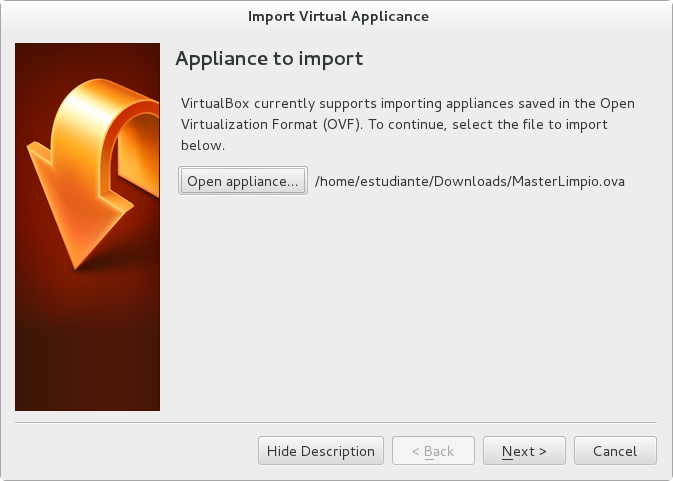
\includegraphics[width=0.5\textwidth]{aux/importappliance}


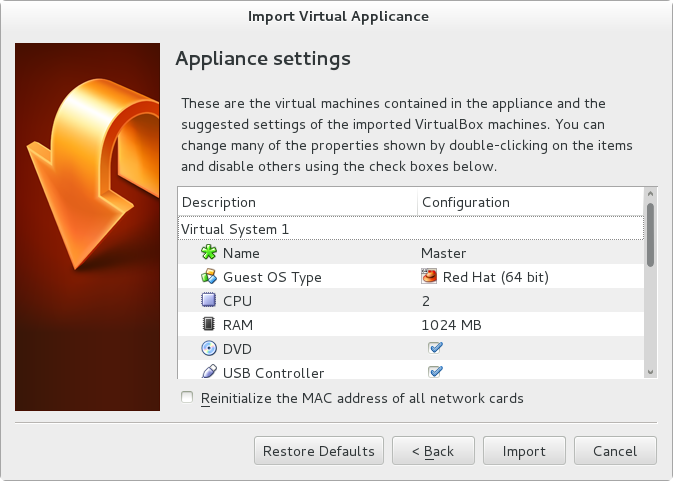
\includegraphics[width=0.5\textwidth]{aux/applianceops1}

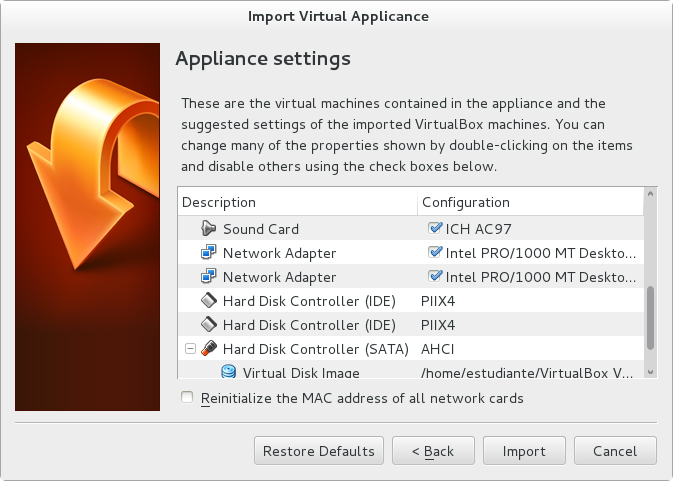
\includegraphics[width=0.5\textwidth]{aux/applianceops2}


\item Señale la máquina virtual llamada ``Master'' y vaya a la configuración y revise la siguiente configuración en esta:

\begin{itemize}

	\item En la sección Sistema, pestaña Procesador, debe tener dos procesadores y habilitado PAE/NX.

	
	
	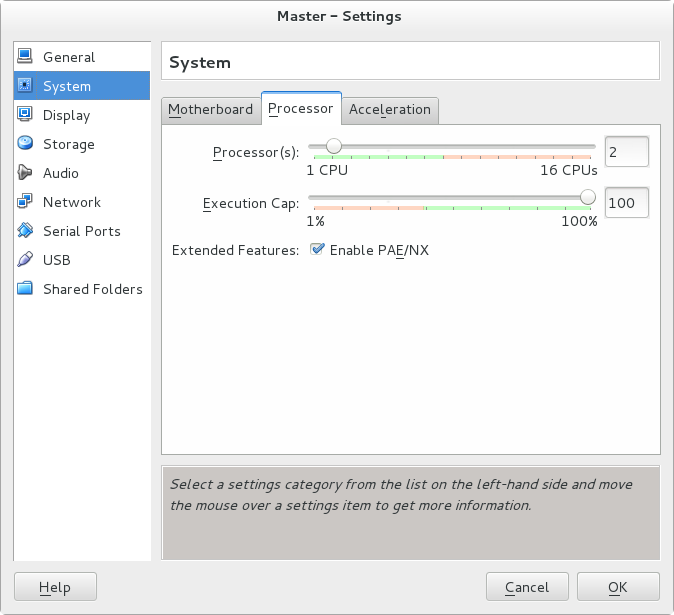
\includegraphics[width=0.5\textwidth]{aux/procesadores}
	

	\item En la sección Red, pestaña Adaptador 1, deberá estar configurado como NAT. 


	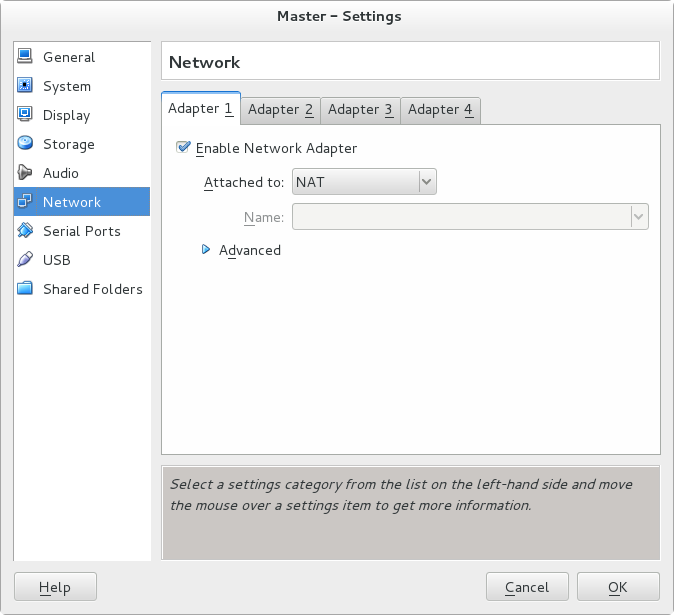
\includegraphics[width=0.5\textwidth]{aux/rednat}
	

	\item En la pestaña Adaptador 2 deberá estar en Adaptador Sólo--Anfitrión y el nombre deberá ser \texttt{vboxnet0}\footnote{Tenga en cuenta que este adaptador se llama \texttt{vboxnet0} en Linux, en Windows tendrá otro nombre, lo más importante es que sea la primera interfaz de red de Sólo Anfitrión, ya que sino dará lugar al problema de reasignación de interfaces de red dentro del nodo Master, en otras palabras, asignará las interfaces eth2 y eth3 en vez de asignar eth0 y eth1 a la NAT y a la Sólo Anfitrión respectivamente.}.


	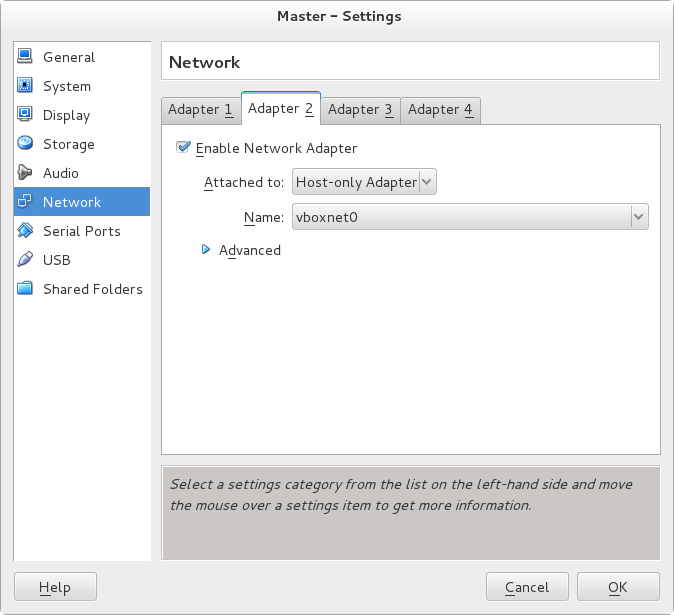
\includegraphics[width=0.5\textwidth]{aux/redhost}
	

	\item Acepte todos los cambios.

\end{itemize}

\item Señale la máquina Master e iníciela.

\item Una vez iniciada la máquina virtual del Master proceda a crear una nueva máquina virtual como Nodo Trabajador a partir de los siguientes pasos:

\begin{itemize}
	\item Haga click en Crear Nueva Máquina.

	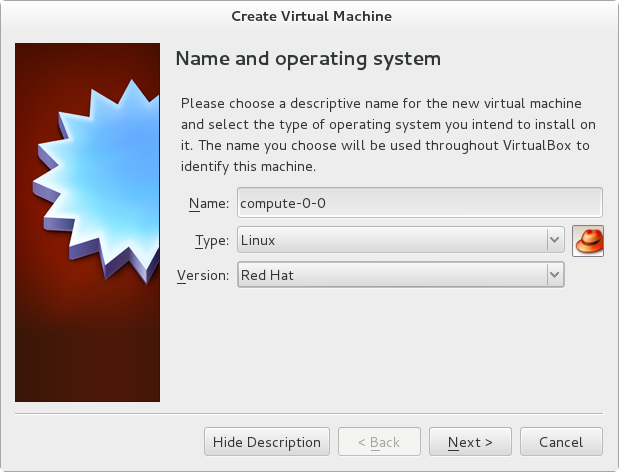
\includegraphics[width=0.5\textwidth]{aux/opcnodo1}

	\item El nombre será \textit{compute-0-0}.

	\item El tipo será Linux.

	\item La versión será Red Hat de 64 bits.

	

	\item Click en siguiente.

	\item Asigne 1024 Megabytes de Memoria RAM\footnote{La cantidad de memoria RAM asignada será proporcional a la que tenga el sistema en el cual están las máquinas virtuales. Igual con el disco duro y los procesadores, sin embargo, para efectos de ver la paralelización en memoria compartida se recomienda tener 2 procesadores por máquina}.

	\item Cree el disco duro con 30 gigas de espacio, recuerde que esto se asignará dinámicamente. El tipo de disco duró será VDI y dinámicamente asignado.



	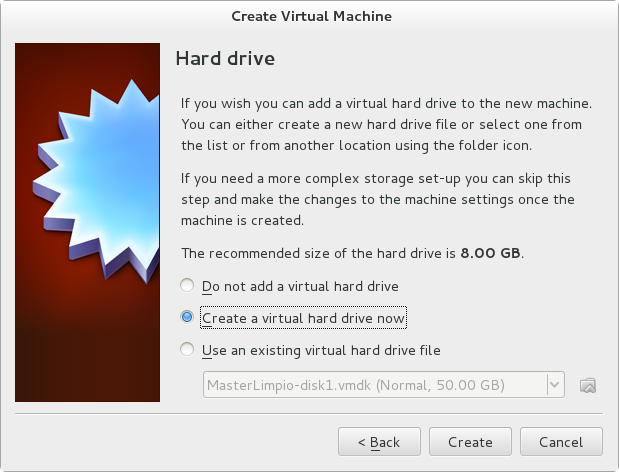
\includegraphics[width=0.5\textwidth]{aux/nodohd}

	
	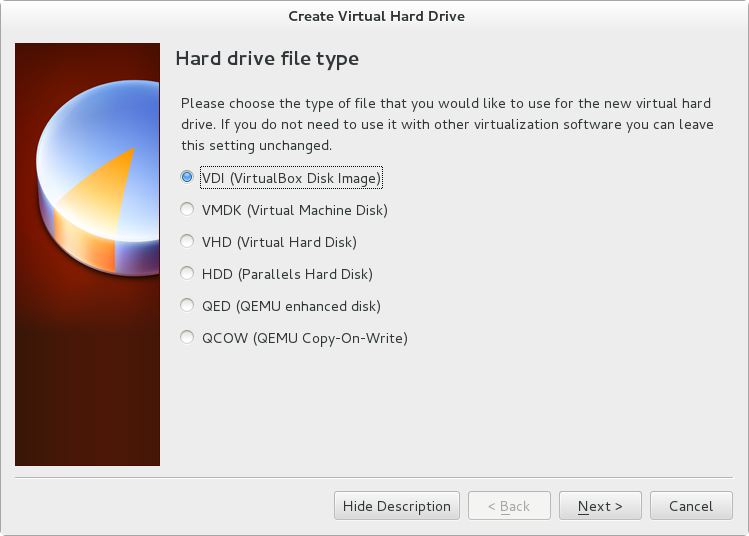
\includegraphics[width=0.5\textwidth]{aux/nododvi}


	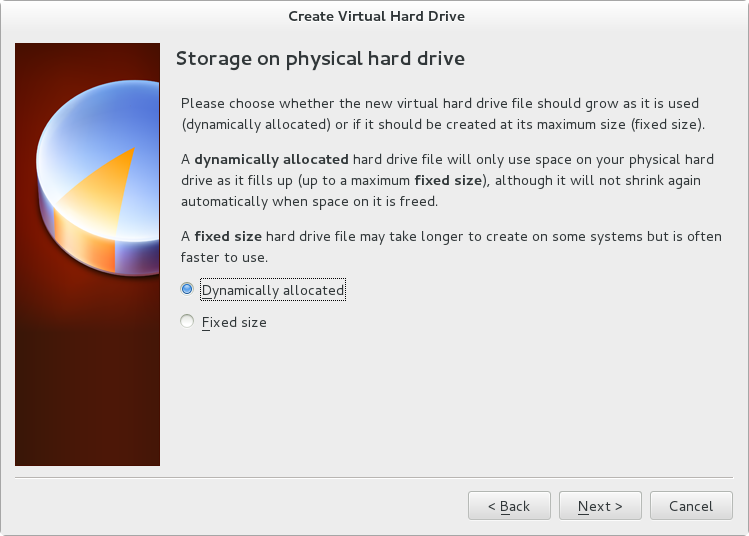
\includegraphics[width=0.5\textwidth]{aux/hddinamico}


	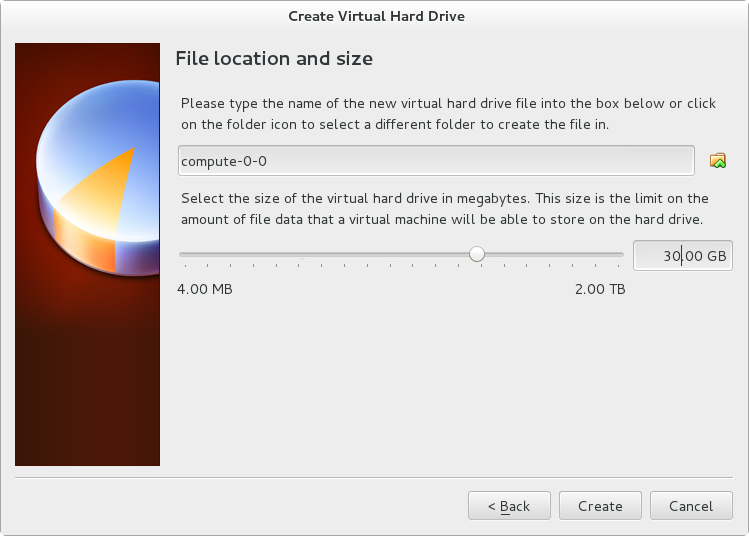
\includegraphics[width=0.5\textwidth]{aux/nodohdsize}
	

\end{itemize}

\item Una vez creado el nodo trabajador se procede a configurarlo a partir de los siguientes pasos:

\begin{itemize}
	\item Señalar la máquina \textit{compute-0-0} y dar click en Configurar.

	\item En la pestaña Sistema, asegúrese de que tenga la cantidad de memoria RAM correcta

	\item Deshabilite el \textit{floppy disk}

	\item habilite la red como dipositivo de \textit{booteo} y además súbalo como primer dispositivo, sólo deberá quedar la tarjeta de red como primera opción y como segunda el disco duro de la máquina virtual, de esta manera nos aseguramos que esta máquina virtual pueda instalarse automáticamente de manera desatendida, por esta razón el clúster es escalable. 

	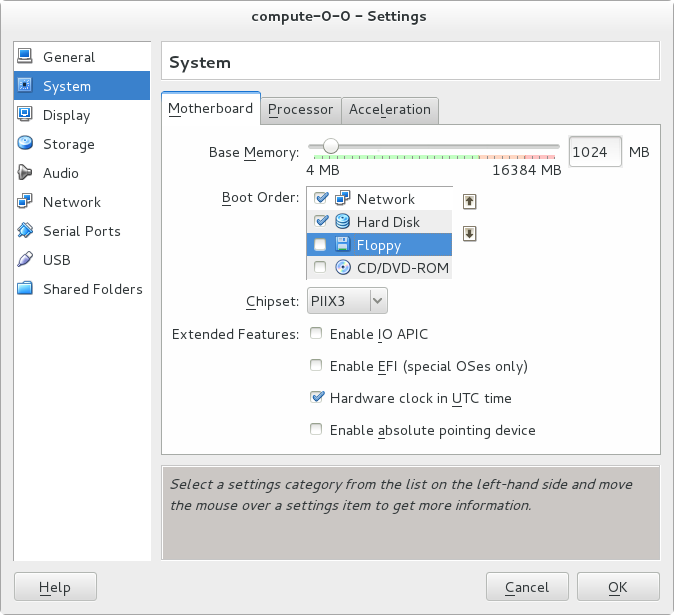
\includegraphics[width=0.5\textwidth]{aux/nodoopsboot}


	\item En la pestaña Procesador asegúrese de que hay dos procesadores y está habilitado PAE/NX.


	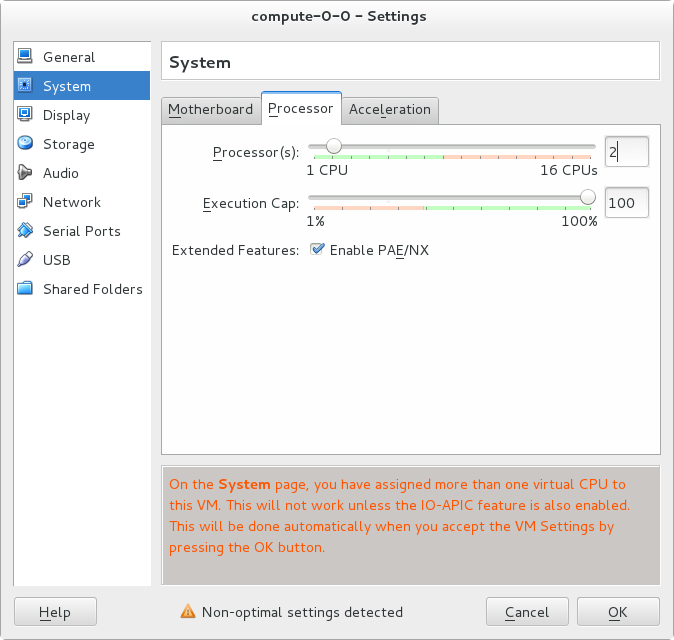
\includegraphics[width=0.5\textwidth]{aux/nodoprocesadores}
	

	\item En la sección Red deberá configurar sólo la primera interfaz de red y deberá estar configurada como Sólo--Anfitrión y deberá tener \texttt{vboxnet0}.


	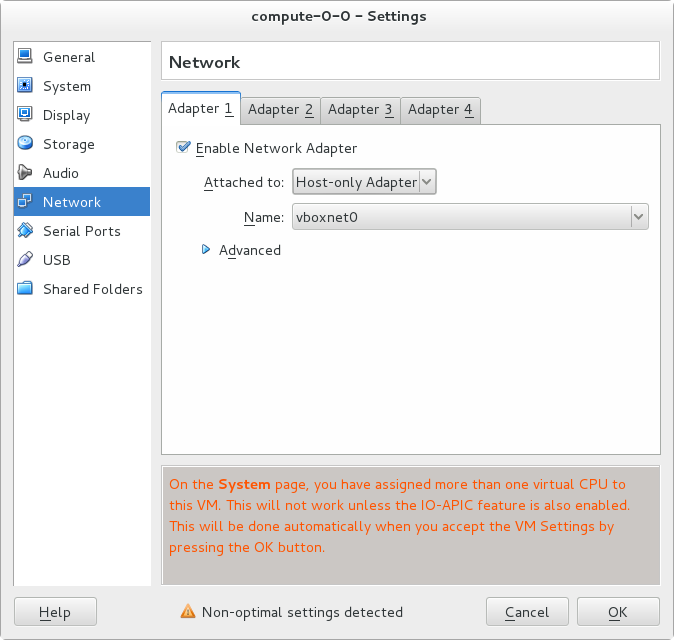
\includegraphics[width=0.5\textwidth]{aux/nodored}
	

	\item Acepte los cambios.
\end{itemize}


\item Repita los pasos para crear otro nodo si lo considera necesario para crear el \textit{compute-0-1}, siempre y cuando la computadora que usted tiene soporte una tercera máquina virtual ejecutandose al tiempo que el Nodo Master y el \textit{compute-0-0}

\item Ingrese en el Nodo Master como usuario \texttt{root} y la contraseña es \texttt{apolito123!}

\item Abra una consola

\item Ingrese el comando \texttt{insert-ethers}

\item Escoja \texttt{Compute}. Aparecerá una interfaz de consola mostrándole los nodos agregados en la medida que se les vaya asignando IP por medio de DHCP y una imagen de Linux para instalar con PXE.

\item Encienda de uno en uno los Nodos trabajadores que haya creado, empezando por el \textit{compute-0-0} y así sucesivamente. Observará que aparece en la interfaz \texttt{insert-ethers} la dirección MAC del Nodo Trabajador, se le asignará el nombre compute-0-0 y si aparece un símbolo de asterísco es porque recibió exitosamente la imagen para la instalación de Linux.

\item Una vez de que los nodos se termine de instalar automáticamente salga de la interfaz de \texttt{insert-ethers} en el Master con la tecla F8.

\item Ingrese al directorio especificado con el siguiente comando: \texttt{cd /export/apps/installers}

\item Descargue el instalador del comando \texttt{htop} con la siguiente instrucción: \texttt{wget http://goo.gl/TDWExw}

\item Instale \texttt{htop} en el nodo Master con la siguiente instrucción: \texttt{rpm -ivh htop*.rpm}

\item Ahora instale masivamente \texttt{htop} en el resto del clúster con el siguiente comando: \texttt{rocks run host ``rpm -ivh /share/apps/installers/htop*.rpm''}

\item El cluster está completo.

\end{enumerate}

\subsection{Configuración de los Nodos Esclavos}

\begin{enumerate}
	\item Una vez que se tiene el nodo Master funcionando y por lo menos un nodo trabajador como el \textit{compute-0-0} se procede a realizar los siguientes pasos de configuración:

	\begin{itemize}
	\item Adicione un usuario sin privilegios con los siguientes comandos\footnote{En adelante el usuario de ejemplo será jdpinedac, pero usted podrá asignar el nombre de usuario que desee}:

	\begin{itemize}
		\item \textbf{\texttt{adduser jdpinedac}} Para crear un usuario sin privilegios.

		\item \textbf{\texttt{passwd jdpinedac}} Para cambiar la contraseña del usuario.

		\item \textbf{\texttt{rocks sync users}} Para sincronizar el usuario creado en todo el cluster, este usuarió estará creado tanto en el nodo master como en los nodos trabajadores.
	\end{itemize}

	\item \textit{su - jdpinedac} Para que el usuario \texttt{root} se convierta en el usuario sin privilegios. Se le harán algunas preguntas de contraseñas, déjelas vacías presionando la tecla \textit{enter} varias veces.
	\end{itemize}
	
\end{enumerate}


\section{Preguntas Frecuentas:}[Posibles Problemas]

\begin{itemize}
	\item Los nodos de trabajo no inician Correctamente: Es posible que estos hayan sido apagados de manera incorrecta. 
	siga el procedimiento desde el numeral X hasta el Y de ``ASDF''

	\item Verifique que su computador puede virtualizar: Ingrese a la BIOS y verifique que esta activida la opcion de Virtualización de Hardware. 

	\item Si su caso no se encuentra aqui listado contacte al autor
\end{itemize}

\chapter{Instalación}
Ejemplo Programa Corriendo en Apolo

Programa Normal. 

Ejecturar


Instalacion de Boost


Repast HPC
wget http://repast.sourceforge.net/hpc_tutorial/SRC.tar.gz
tar xvf SRC.tar.gz

rocks run host rmpb -ivh /export/apps/installers/*.rpm


Agregar usuario sin privilegios. 

adduser smonsalve
passwd smonsalve
rocks sync users


insert-ethers --remove compute-0-0
insert-ethers --remove compute-0-1
insert-ethers 

rocks run host hostname
rocks run host poweroff



Debido a las relaciones de confianza entre el master y los nodo


ssh compute-0-0
ssh compute-0-1


Para monitorear la actividad del master y los nodos podemos utiliar el programa htop, el cual se encarga de mostrarnos los procesos, las cpus y los cores disponibles dentro del nodo. 



\chapter{Ejecución}
Contando ya con el ambiente necesario para la ejecución del código a paralelizar se procede a realizar los siguientes pasos: 

\begin{enumerate}

	\item Desde la maquina virtual del master abrir una consola. 

	\item Se procede a loggearse como el usuario sin privilegios que se creo (smonsalve) a través de ssh:

	\begin{verbatim}
	$ ssh smonsalve@192.168.56.101
	\end{verbatim}

	\item Procedemos a descargar el Código Fuente a ejecutar: 

	\begin{verbatim}
	$ wget goo.gl 
	\end{verbatim}
	

	%\lstinputlisting[label=nodes.txt,caption=Lista de Cores para Ejecutar]{code/breadth_first_search.cpp}


	\item Para compilar este codigo es necesario:


	\begin{verbatim}
	$ mpi
	\end{verbatim}
	

	\todo[inline,caption={TODO}]{source}

	\item También se deben descargar los respectivos datos de entrada: 

	\begin{verbatim}
	$ wget goo.gl
	\end{verbatim}
	

	%\lstinputlisting[label=nodes.txt,caption=Lista de Cores para Ejecutar]{code/weighted_graph.gr}
	

	\item Es también necesario contar con un archivo que le indique al proceso en que nodos y que cores se va ejecutar el archivo en nuestro caso, un archivo llamado nodos.txt:

	\lstinputlisting[label=nodes.txt,caption=Lista de Cores para Ejecutar]{code/nodes.txt}

	\item para ejecutar finalmente con MPI: 


	\begin{verbatim}
	$ mpirun -n 4 -machinefile nodes.txt \
	> breadth_first_search < weighted_graph.gr
	\end{verbatim}
	
	\item Debido a las relaciones de confianza entre el master y los nodos, desde el master podemos pasar por ssh a los nodos a través del siguiente comando: 

	\begin{verbatim}
	$ ssh compute-0-0
	\end{verbatim}


	\item Desde allí se podrá monitorear la actividad del master y los nodos, para lo cual se puede utilizar el programa ``htop'', el cual se encarga de mostrar los procesos, las CPUs y los cores disponibles dentro del nodo. 

	\item  Desde cada uno de los nodos se abre ``htop'' para monitorear que se esté procesando en todos los nodos y en cada core de los cores, en este caso, dos nodos con dos cores cada uno:   


	\begin{verbatim}
	$ htop
	\end{verbatim}

	\begin{verbatim}
	$ ssh compute-0-1
	\end{verbatim}

	\begin{verbatim}
	$ htop
	\end{verbatim}

	\todo[inline,caption={TODO}]{imagen htop}

	% \begin{figure}[H]
	% 	\centering
	% 	\includegraphics[width=0.5\textwidth]{aux/}
	% 	\caption[]{}
	% 	%(tomada de \cite{WikiEmotion)}
	% 	%\label{F-dimensions-emotion}
	% \end{figure}


	\item Para volver al Master se escribe el comando ``exit''


	\begin{verbatim}
	$ exit
	\end{verbatim}

	\item Donde se podrán ver los datos de Salida en el mismo directorio donde se ejecuto el programa desde el master. Si  se verifica el contenido del directorio debe aparecer el archivo de salida generado, con el nombre: ``weighted\_graph-bfs.dot''

	 \begin{verbatim}
	 (master)$ ls 
	 \end{verbatim}


	 % \begin{figure}[H]
	 % 	\centering
	 % 	\includegraphics[width=0.5\textwidth]{aux/}
	 % 	\caption[]{}
	 % 	%(tomada de \cite{WikiEmotion)}
	 % 	%\label{F-dimensions-emotion}
	 % \end{figure}
	 

	\item De esta manera se puede observar que el programa ``bfs'' se ejecuto de la manera deseada, produciendo como resultado el respectivo archivo de salida, resultado de un proceso paralelizado.


\end{enumerate}
 

\chapter{Conclusiones}
Conclusiones

\chapter{Trabajo Futuro}
Adicional a las posibilidades de uso de este proyecto planteadas en la Justificación y posibles aplicaciones, se desea continuar con este proyecto en aplicación a la solución de problemas reales. 

Dentro de las nuevas posibilidades se abren para continuar se destacan: 

\begin{itemize}
	\item Realizar un análisis de un grafo con gran cantidad de datos.
	
	\item Realizar un estudio del rendimiento de un programa con una implementación de Boost en Apolo.

	\item Agregar una sección para el manejo de colas en el clúster. (Torque o PBS )  
	
	\todo[inline,caption={TODO}]{referencias}

\end{itemize}

\chapter{Glosario}
	\label{chapGlosario}

	\begin{description}
		\item[HPC:] (High Performance Computing) Computación de alto desempeño.
		\item[Data Center:]
	\end{description}

\newpage

\bibliography{Tesis}

\bibliographystyle{plain}	
	aca
	\cite{czarnecki2000generative}
	\cite{wwwBoost}
	\cite{stroustrup2013c++}
	\cite{andrei2001modern}
	\cite{Wall2000}
	\cite{Boost}
	\cite{Karniadakis}
	\cite{Kernighan1988}

\newpage

\appendix

\chapter{Repositorio del código}

	Para una copia del código utilizado dirigirse a: \url{https://github.com/smonsalve/tesis.git}

	OVA de la maquina virtual con Rocks instalado y dos nodos.

	Input data para Grafo (X Vertices y Y Aristas).

	Makefile de Instalación.

\end{document}
